% ju 28-Mai-22
\documentclass[a4paper,12pt,fleqn,parskip=half]{scrartcl}
\usepackage[ngerman]{babel}
\usepackage[utf8]{inputenc}
\usepackage[T1]{fontenc}

% Schrift
%\usepackage{lmodern}
\usepackage[osf,sc]{mathpazo} 
\usepackage[scale=.9,semibold]{sourcecodepro}   
\usepackage[osf]{sourcesanspro}  

\usepackage[headsepline]{scrlayer-scrpage}
\pagestyle{scrheadings}
\clearpairofpagestyles

\usepackage[table,dvipsnames,usenames]{xcolor}
\usepackage{textcase}
\usepackage{nameref}
\usepackage{hyperref}
\usepackage{tabularx}
\usepackage{multirow}
\usepackage{multicol}
\usepackage{caption, booktabs}
\usepackage{graphicx} 
\usepackage{scrhack}    
\usepackage{url}%% Links
\usepackage[inline]{enumitem}
\usepackage{pifont}
\usepackage{eurosym}% \euro 20,-
\usepackage{amsmath}
\usepackage{amsfonts}
\usepackage{amssymb}
\usepackage{array}            % Extending the array and tabular environments
\usepackage{chngcntr}         % Change the resetting of counters
\usepackage[version=4]{mhchem}
\usepackage{stmaryrd}
\usepackage{siunitx}
\usepackage{float}
\usepackage{csquotes}
\usepackage{subcaption}
\usepackage{mathtools}
\usepackage{icomma}%Dezimaltrennzeichen
\usepackage{multimedia}%Video: \movie[externalviewer]{(video.mov)}{video.mov}
\usepackage{epstopdf}
\usepackage{footnote}
\usepackage{qrcode}% Anwendung: \qrcode[hyperlink,level=Q,version=2,height=1cm]{\website}
\usepackage{underscore}% Unterstrich ____

% PDF Dokumente einbinden
\usepackage{pdfpages}% \includepdf[pages=-]{Tabellen/Excel.pdf}
\RequirePackage{lastpage}  % Pagecounter

\addto\captionsngerman{%
\renewcommand{\figurename}{Abb.}
\renewcommand{\tablename}{Tab.}
}

% listings
\usepackage{listings}
\lstset{basicstyle=\linespread{1}\ttfamily\small,floatplacement=!htb,captionpos=t,abovecaptionskip=.5\baselineskip,belowcaptionskip=.5\baselineskip,upquote=true,showstringspaces=false,inputencoding=utf8,tabsize=4,
    	keywordstyle=\bfseries ,
	commentstyle=\color{rot5},
	stringstyle=\color{orange},
	breaklines=true,
  	postbreak=\mbox{\textcolor{black}{$\hookrightarrow$}\space},
	breakatwhitespace=false
}
\lstset{literate={á}{{\'a}}1 {é}{{\'e}}1 {í}{{\'i}}1 {ó}{{\'o}}1 {ú}{{\'u}}1 {Á}{{\'A}}1 {É}{{\'E}}1 {Í}{{\'I}}1 {Ó}{{\'O}}1 {Ú}{{\'U}}1 {à}{{\`a}}1 {è}{{\`e}}1 {ì}{{\`i}}1 {ò}{{\`o}}1 {ù}{{\`u}}1 {À}{{\`A}}1 {È}{{\'E}}1 {Ì}{{\`I}}1 {Ò}{{\`O}}1 {Ù}{{\`U}}1 {ä}{{\"a}}1 {ë}{{\"e}}1 {ï}{{\"i}}1 {ö}{{\"o}}1 {ü}{{\"u}}1 {Ä}{{\"A}}1 {Ë}{{\"E}}1 {Ï}{{\"I}}1 {Ö}{{\"O}}1 {Ü}{{\"U}}1 {â}{{\^a}}1 {ê}{{\^e}}1 {î}{{\^i}}1 {ô}{{\^o}}1 {û}{{\^u}}1 {Â}{{\^A}}1 {Ê}{{\^E}}1 {Î}{{\^I}}1 {Ô}{{\^O}}1 {Û}{{\^U}}1 {œ}{{\oe}}1 {Œ}{{\OE}}1 {æ}{{\ae}}1 {Æ}{{\AE}}1 {ß}{{\ss}}1 {ű}{{\H{u}}}1 {Ű}{{\H{U}}}1 {ő}{{\H{o}}}1 {Ő}{{\H{O}}}1 {ç}{{\c c}}1 {Ç}{{\c C}}1 {ø}{{\o}}1 {å}{{\r a}}1 {Å}{{\r A}}1 {€}{{\EUR}}1 {£}{{\pounds}}1 {~}{{\textasciitilde}}1 {-}{{-}}1 }

% bibliography
\usepackage[
    bibencoding=utf8,
    backend=biber,% bibtex, biber
    backref=false,backrefstyle=three+,url=true,urldate=comp,abbreviate=false,maxnames=20
]{biblatex} %Paket laden
\DeclareBibliographyCategory{cited}
\let\defaultcite\cite\renewcommand*\cite[2][]{\addtocategory{cited}{#2}\defaultcite[#1]{#2}}
\let\defaulttextcite\textcite\renewcommand*\textcite[2][]{\addtocategory{cited}{#2}\defaulttextcite[#1]{#2}}
\setcounter{biburllcpenalty}{7000}
\setcounter{biburlucpenalty}{8000}
\AfterPackage{biblatex}{
	\PreventPackageFromLoading[\errmessage{Sie haben versucht, das Cite-Paket zu laden, das nicht mit biblatex kompatibel ist.}]{cite}
}

\hypersetup{%
	%pdftitle={\titel},
	%pdfsubject={Latex},
	%pdfauthor={\autor},
	%pdfcreator={\autor}, 
	bookmarksnumbered=true,
	breaklinks=true,
	%colorlinks=true,	   
	linkcolor=rot5,		
	filecolor=blau5,		
	urlcolor=blau5,			
	citecolor=ForestGreen
}

\linespread{1.1}
\setlist{itemsep=0pt}
\widowpenalty10000
\clubpenalty10000
\tolerance1000   

\usepackage[left=2cm,right=2cm,top=1cm,bottom=1cm,includeheadfoot]{geometry}
%\usepackage[left=4cm,right=2cm,top=1cm, bottom=1cm,includeheadfoot]{geometry}
%\usepackage[left=6cm,right=1cm,top=1cm, bottom=1cm,includeheadfoot]{geometry}
%\usepackage[landscape=true,left=2cm,right=2cm,top=1cm,bottom=1cm,includeheadfoot]{geometry}%quer

% eigene Farbe definieren
% Adobe Prozessfarben: CMYK: 100,50,0,35 -> 1,0.5,0,0.35
\definecolor{orange}{cmyk}{0,0.55,0.61,0}   % 0,55,61,0
\definecolor{blau5}{cmyk}{1,0.77,0.1,0.01}  % 100,77,10,
\definecolor{rot5}{cmyk}{0.22,1,1,0.19}     % 22,100,100,19
\definecolor{grau2}{cmyk}{0,0,0,0.1}        % 0,0,0,40
\definecolor{blau}{cmyk}{0.93,0.66,0,0.21}% 

% Literatur
\bibliography{content/literatur}
\bibliography{content/literatur-kfz}
\bibliography{content/literatur-sport}

%%%%%%%%%%%%%%%%%%%%%%%%%%%%%%%%%%%%%%%%%%%%%%%%%%%%%%%
\newcommand{\name}{Jan Unger}% anpassen!!!!!
\newcommand{\thema}{FM_U02_Leiterwiderstand_Loesung}
\newcommand{\quelle}{\name}
\newcommand{\website}{https://bw-ju.de/}
\newcommand{\github}{https://github.com/ju1-eu}
%%%%%%%%%%%%%%%%%%%%%%%%%%%%%%%%%%%%%%%%%%%%%%%%%%%%%%%

\ihead{\textbf{Quelle:} \quelle}%{Kopfzeile innen}
\ohead{\textbf{Datum:} \today}  %{Kopfzeile außen}

\ifoot{\textbf{Thema:} \thema}  %{Fußzeile  innen}
\ofoot{Seite {\thepage} von {\pageref{LastPage}}}%{Fußzeile  außen}

\title{\thema}
\author{\name}
\date{\today}

\begin{document}
	%\thispagestyle{empty}
	%\maketitle
	%\newpage
	%\setcounter{page}{1}

	%%%%%%%%%%%%%%%%%%%%%%%%%%%%%%%%%%%%%%%%%%%
	\begin{center}
		\textbf{\Large \thema}%14pt
		\vspace{0.8em}
		
		%\datum	
		%\qrcode[hyperlink,level=Q,version=2,height=1cm]{\website}
		\qrcode[hyperlink,level=Q,version=2,height=1cm]{\github}
	\end{center}
	%%%%%%%%%%%%%%%%%%%%%%%%%%%%%%%%%%%%%%%%%%%

	\subsection*{Keywords}%\label{sec:Deadline}\index{Deadline}
	% Checkliste
	\begin{itemize}[label=\checkmark] %\itemsep -2pt
		\item Begriff 
	\end{itemize}

    %%%%%%%%%%%%%%%%%%%%%%%%%%%%%%%%%%%%%%%%%%%%%%%%%%%%%%%%%%%%%%%%%%

	% anpassen
	%\input{content/tex/neu}
	%ju 28-Mai-22 FM_U02_Leiterwiderstand_Loesung.tex
\section{Leiterwiderstand Übung 2}\label{leiterwiderstand-uebung-2}

\textbf{Aufgabe 1}

geg:

$l = 8,25~m$

$A = 0,75~mm^2$

$\rho = 0,0178~\frac{\Omega \cdot mm^2}{m} \,\text{(Kupfer)}$

ges: $R_l$

Formel

$R_l = \frac{p \cdot l}{A}$

Lösung

$R_l = 0,1958~\Omega$

\textbf{Aufgabe 2}

geg:

$R_l = 0,3648~m\Omega = 0,0003648~\Omega = \num{3,648e-04}~\Omega$

$\rho = 0,0178~\frac{\Omega \cdot mm^2}{m} \,\text{(Kupfer)}$

$d = 12,363~mm$

ges: $A, l$

Formel

$A = d^2 \cdot \pi$ oder $A = d^2 \cdot 0,785 \to (pi/4 = 0,785)$

$R_l = \frac{p \cdot l}{A} \to l = \frac{R_l \cdot A}{p}$

Lösung

$l = 2,459~m$

\textbf{Aufgabe 3}

geg:

$l = 4,5~m$

$R_l = 0,00267~\Omega = 2,666666~m\Omega = \num{2,67e-03}~\Omega$

$\rho = 0,0178~\frac{\Omega \cdot mm^2}{m} \,\text{(Kupfer)}$

ges: $A$

Formel

$R_l = \frac{p \cdot l}{A} \to A = \frac{p \cdot l}{R_l}$

Lösung

$A = 30,0~mm^2$

\textbf{Aufgabe 4}

\begin{figure}[!ht]% hier: !ht
\centering
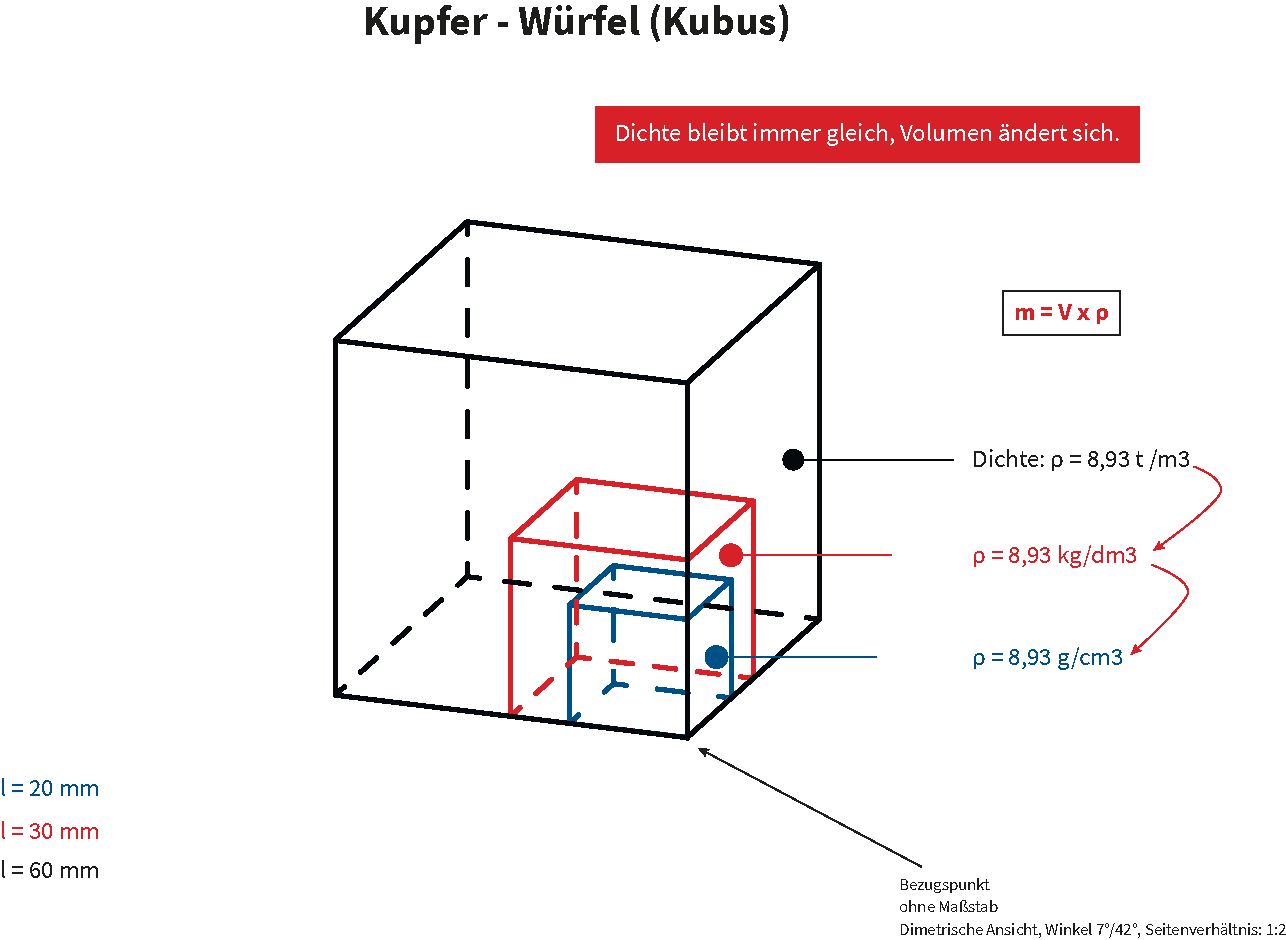
\includegraphics[width=0.6\textwidth]{images/Skizze/Kupfer_Wuerfel_Dichte.pdf}
\caption{Dichte / Volumen eines Kupferwürfels}
%\label{fig:}%% anpassen
\end{figure}

$\boxed{l = 2~cm}, V = (2~cm)^3 = 8~cm^3$

$m = 8~cm^3 \cdot 8,93~\frac{g}{cm^3} = 71~g$

$\boxed{l = 3~cm} = 0,3~dm, V = (0,3~dm)^3 = 0,027~dm^3$

$m = 0,027~dm^3 \cdot 8,93~\frac{kg}{dm^3} = 0,241~kg = 241~g$

$\boxed{l = 6~cm} = 0,06~m, V = (0,06~m)^3 = 0,000216~m^3$

$m = 0,000216~m^3 \cdot 8,93~\frac{t}{m^3} = 0,001929~t = 1929~g$

geg: Spule

$d_m = 36~mm = 3,6~cm$

$N = 1480$ (Windungen)

$d_D = 0,36~mm$

$p_{cu} = 8,93~\frac{t}{m^3}$ (Dichte)

$\rho = 0,0178~\frac{\Omega \cdot mm^2}{m} \,\text{(Kupfer)}$

ges: $A, l, R_l, G, V, m$

Formel

\emph{Kreisringfläche}: D = Außendurchmesser; d = Innendurchmesser; r =
Radius; $d_{mitte} = d_m$

$U = d \cdot \pi; \quad d_m = \frac{(D+d)}{2}; \quad r_m = \frac{(D+d)}{4}$

$A = \frac{d_D^2 \cdot \pi}{4}$

$l = U \cdot N \to l = \frac{d_m}{10} \cdot \pi \cdot N$

$R_l = \frac{\rho \cdot l}{100 \cdot A}$

$G = \frac{1}{R_l}$

$V = A \cdot h \to V = \frac{A}{100} \cdot l$

$m = V \cdot p_{cu}$

Lösung

$A = 0,1018~mm^2$

$l = 16738,4057~cm$

$R_l = 29,2711~\Omega$

$G = 0,0342~S$

$V = 17,0376~cm^3$

$m = 152,146~g$

\textbf{Aufgabe 5,1}

geg:

$R_l = 13,171999~m\Omega = 0,013171999~\Omega = \num{1,3171999e-2}~\Omega$

$\rho = 0,0178~\frac{\Omega \cdot mm^2}{m} \,\text{(Kupfer)}$

$d = 1,784576526~mm$

ges: $A, l$

Formel

$A = d^2 \cdot 0,785 \to (pi/4 = 0,785)$

$R_l = \frac{\rho \cdot l}{A} \to l = \frac{R_l \cdot A}{\rho}$

Lösung

$l = 1,85~m$

\textbf{Aufgabe 5,2}

Gleiche Leiterfläche für die Rückleitung, dass sie genauso hoch belastet
wird wie die positive Versorgungsleitung,

Sie liegen beide in Reihe, werden also vom gleichen Strom durchflossen,


	%%%%%%%%%%%%%%%%%%%%%%%%%%%%%%%%%%%%%%%%%%%%%%%%%%%%%%%%%%%%%%%%%%
    % Bibliographie
    \printbibliography
\end{document}
